\section{Вычислительный эксперимент}

Цель вычислительного эксперимента --- проверить качество предлагаемого метода дистилляции,
проанализировать получившиеся модели и их зависимость от гиперпараметров.

Все методы оцениваются на датасетах для классификации изображений: CIFAR-10 \cite{Krizhevsky2009LearningML}  и Fashion-MNIST \cite{xiao2017fashion}.
CIFAR-10 содержит в себе цветные изображения, разбитые на 10 разных классов.
Fashion-MNIST содержит в себе изображения в оттенках серого, разбитые на 10 классов одежды и обуви.

Сравниваются и анализируются в ходе эксперимента следующие методы:

\begin{enumerate}
    \item Оптимизация без дистилляции.
    \item Оптимизация с дистилляцией Хинтона \cite{hinton2015distilling}.
    \item Оптимизация с дистилляцией Sungsoo Ahn \cite{Ahn_2019_CVPR}, то есть:
          $$\lambda_{i,j} = 1 \quad \text{если} \quad i = j,$$
          $$\lambda_{i,j} = 0 \quad \text{если} \quad i \neq j.$$
    \item Предлагаемый метод дистилляции, со всеми связями, то есть $\lambda_{i,j} = 1$.
    \item Предлагаемый метод дистилляции, со случайной инициализацией гиперпараметров $\lambda$.
    \item Предлагаемый метод дистилляции, оптимизируем гиперпараметры, используя вероятностные модели. Для этого метода используем библиотеку Optuna.
\end{enumerate}

Каждый датасет был разделён на тренировочную и тестовую часть. Во всех методах значение гиперпараметра $\beta = 0.5$.
Метрикой качества была выбрана точность.

\begin{figure}[!htbp]
    \centering
    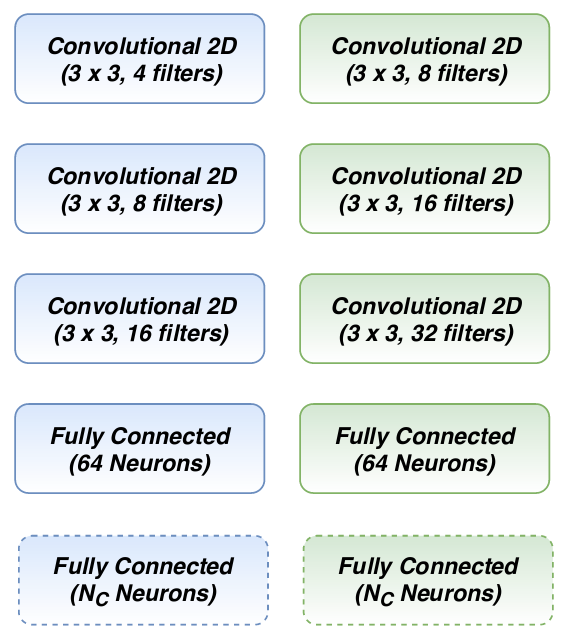
\includegraphics[width=0.5\textwidth]{conv_scheme.png}
    \caption{Архитектура моделей Tiny и VeryTiny}
    \label{fig:model_scheme}
\end{figure}

Как модель учителя использовалась предобученная свёрточная модель под именем Tiny, которая состоит из трёх свёрточных слоёв, и двух линейных.
В качестве ученика использовалась модель под именем VeryTiny, которая отличается от Tiny уменьшенным в два раза количеством каналов в свёрточных слоях.
Архитектура моделей изображена на рисунке \ref{fig:model_scheme}.

Во всех алгоритмах шаг градиентного спуска был равен $0.1$, обучение длилось $50$ эпох.


\begin{table}[h!]
    \centering
    \caption{Значение качества экспериментов на датасетах CIFAR-10 и Fashion-MNIST}
    \begin{tabular}{|c|c|c|}
        \hline
        Метод                                & CIFAR-10 & Fashion-MNIST \\
        \hline \hline
        Без дистилляции                      & $0.541$  & $0.839$       \\ \hline
        Дистилляция Хинтона                  & $0.563$  & $0.849$       \\ \hline
        Дистилляцией Sungsoo Ahn             & $0.591$  & $0.852$       \\ \hline
        Наш метод, все связи                 & $0.590$  & $0.853$       \\ \hline
        Наш метод, случайные гиперпараметры  & $0.595$  & $0.859$       \\ \hline
        Наш метод, вероятностная оптимизация & $0.608$  & $0.857$       \\ \hline
    \end{tabular}
    \label{table:result_accuracy}
\end{table}

\begin{figure}[!htbp]
    \centering
    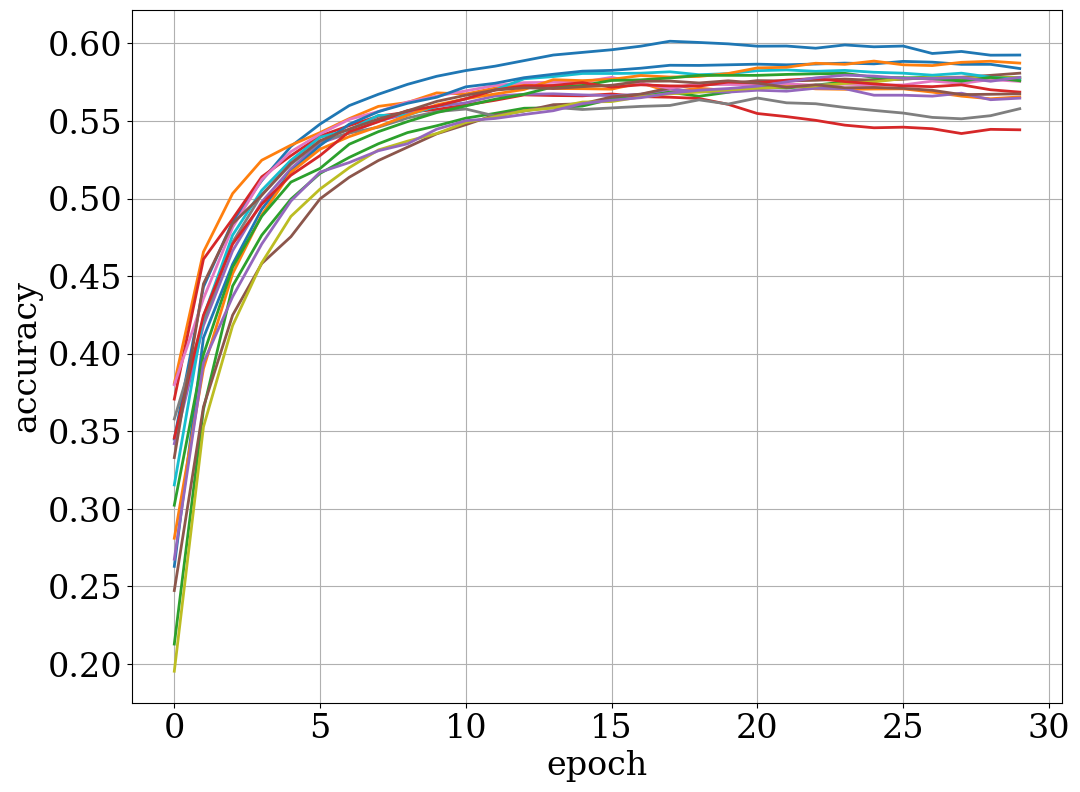
\includegraphics[width=0.9\textwidth]{distill_epoch_accuracy.png}
    \caption{Зависимость качества модели ученика от эпохи на датасете CIFAR-10}
    \label{fig:accuracy_cifar10}
\end{figure}


Финальные результаты продемонстрированы в таблице \ref{table:result_accuracy}. Зависимость качества ученика от эпохи для CIFAR-10 изображена на рисунке \ref{fig:accuracy_cifar10}.

\begin{figure}[H]
    \begin{minipage}[h]{0.35\linewidth}
        \center{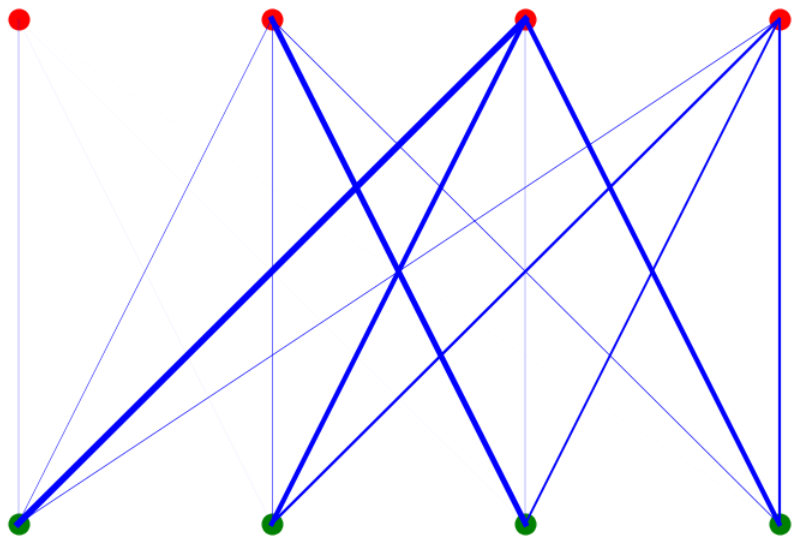
\includegraphics[width=1\linewidth]{connections_1}} \\
    \end{minipage}
    \hfill
    \begin{minipage}[h]{0.35\linewidth}
        \center{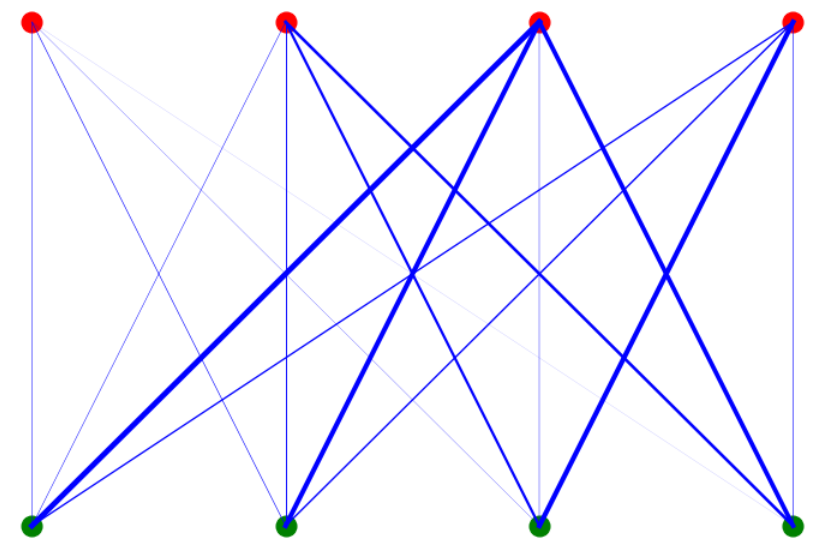
\includegraphics[width=1\linewidth]{connections_2}} \\
    \end{minipage}
    \vfill
    \begin{minipage}[h]{0.35\linewidth}
        \center{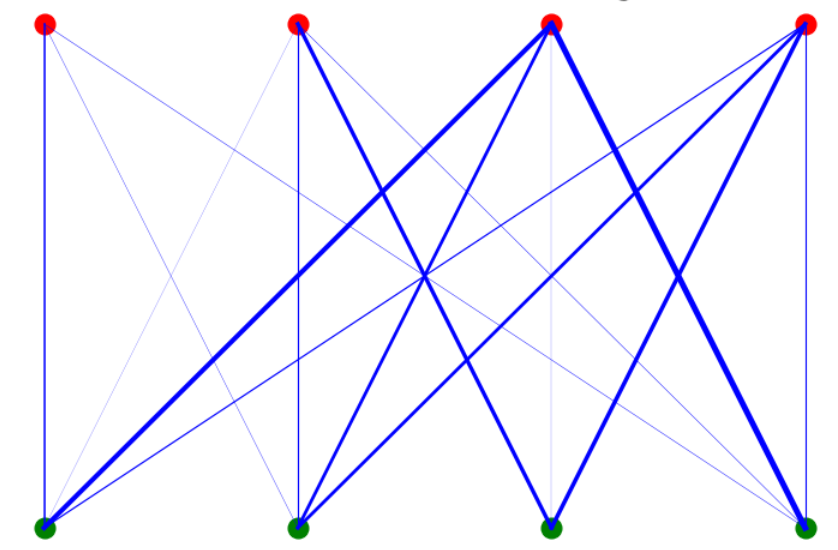
\includegraphics[width=1\linewidth]{connections_3}} \\
    \end{minipage}
    \hfill
    \begin{minipage}[h]{0.35\linewidth}
        \center{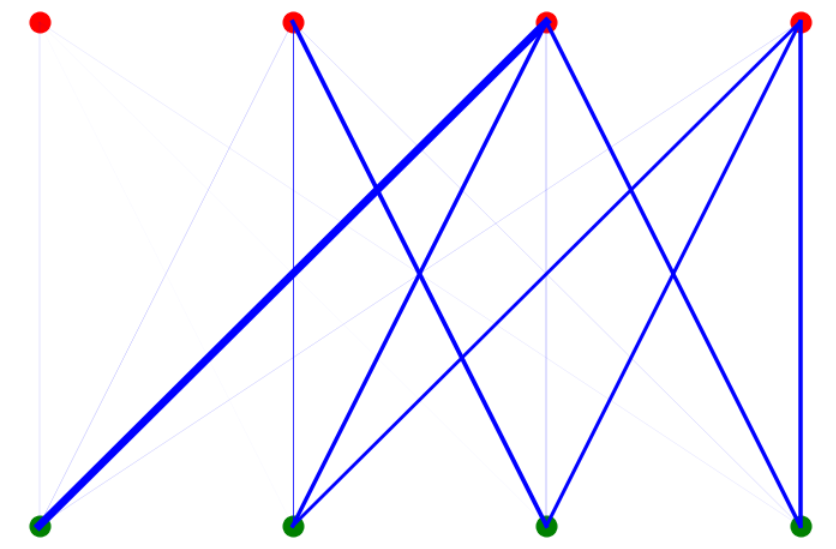
\includegraphics[width=1\linewidth]{connections_4}} \\
    \end{minipage}
    \caption{Иллюстрация коэффициентов у четырех лучших моделей по качеству в эксперименте с случайным подбором гиперпараметров на датасете CIFAR-10.
        Зелёные точки --- слои ученика, красные --- слои учителя. Чем толще линия, тем больше коэффициент $\lambda$ у соответствующей связи.}
    \label{fig:lines}
\end{figure}

Интерес для дальнейших исследований представляет собой связь гиперпараметров $\lambda_{i,j}$ с итоговым качеством модели.
На рисунке \ref{fig:lines} схематически изображены значения коэффициентов $\lambda_{i,j}$ в четырех лучших запусках в эксперименте с случайным подбором гиперпараметров,
на датасете CIFAR-10. Видно некоторую закономерность, что связи, которые ведут к третьему слою учителя, у которого наибольшее число параметров, больше, чем остальные.
В дальнейших исследованиях планируется подробнее изучить связь гиперпараметров и вывести условия или законы, которые связывают их с качеством модели ученика при дистилляции.
